\documentclass{beamer}
%
% Choose how your presentation looks.
%
% For more themes, color themes and font themes, see:
% http://deic.uab.es/~iblanes/beamer_gallery/index_by_theme.html
%

\mode<presentation>
{
  \usetheme{Darmstadt}      % or try Darmstadt, Madrid, Warsaw, ...
  \usecolortheme{beaver} % or try albatross, beaver, crane, ...
  \usefonttheme{default}  % or try serif, structurebold, ...
  \setbeamertemplate{navigation symbols}{}
  \setbeamertemplate{caption}[numbered]
} 

\usepackage[backend=bibtex]{biblatex}
\addbibresource{bibliography.bib}

\usepackage[english]{babel}
\usepackage[utf8x]{inputenc}
\usebackgroundtemplate{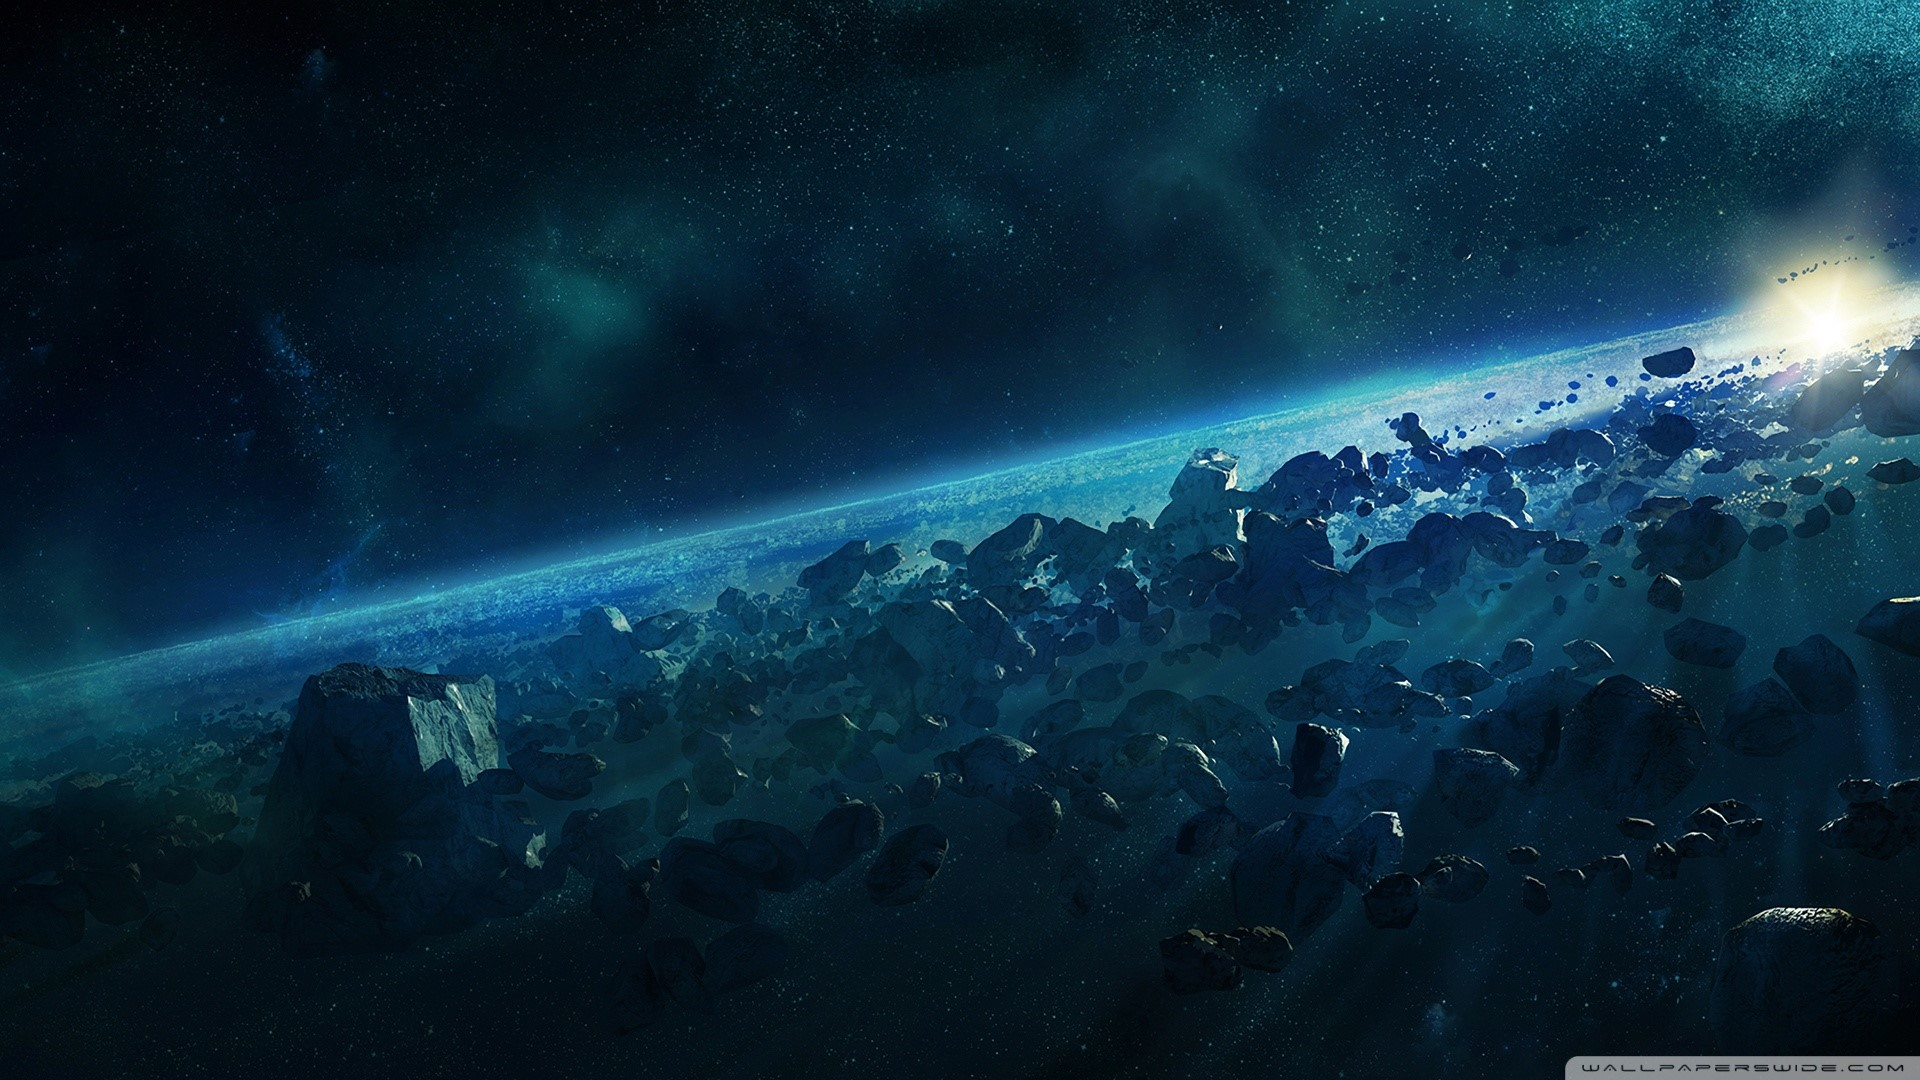
\includegraphics[width=\paperwidth]{Pic/Intro.jpg}}
\title[Hazardous asteroids forecast via Markov random fields]{Hazardous asteroids forecast via Markov random fields}
\subtitle{Project for the exam: Probabilistic Modelling (DSE)}
\author{Marzio De Corato}
\date{\today}

\begin{document}

\begin{frame}
\vspace{+4 cm}  \titlepage
\end{frame}

\usebackgroundtemplate{ } 

% Uncomment these lines for an automatically generated outline.
%\begin{frame}{Outline}
%  \tableofcontents
%\end{frame}

\section{Introduction}

\begin{frame}{Introduction}

\begin{itemize}
\item \textbf{Final Goal} Assessment of forecasts and interpretability for different machine learning algorithms, including the probabilistic models
\item \textbf{Method} Use a dataset for which the laws that interconnects the different features are known from general principles
\item \textbf{Dataset} CNEOS asteroids dataset for more than 3500 asteroids
\item \textbf{Theoretical laws} Celestial mechanics
\item \textbf{Algorithms involved - probabilistic models} GLASSO, mgm, minforest, mmod
\item \textbf{Algorithms involved - others} Random forest, Support Vector Machines, Quadratic Discriminant Analysis, Logistic Regression  

\end{itemize} 

\end{frame}

\section{Celestial mechanics}

\begin{frame}{Celestial mechanics}
\begin{equation}
\textbf{F}_{1}=\mathcal{G} \cdot \frac{m_{1}m_{2}}{r^{3}}\textbf{r}=m_{1} \ddot{\textbf{r}}_{1}
\end{equation}

\begin{equation}
\textbf{F}_{2}=-\mathcal{G} \cdot \frac{m_{1}m_{2}}{r^{3}}\textbf{r}=m_{1} \ddot{\textbf{r}}_{2}
\end{equation}
 
If we consider the motion of the second item with respect to the first one 
 
\begin{equation}
\ddot{\textbf{r}}=\ddot{\textbf{r}}_{2}-\ddot{\textbf{r}}_{1} \quad \mu=\mathcal{G}(m_{1}+m_{2})
\end{equation}

\begin{equation}
\dfrac{d^{2}\textbf{r}}{dt^{2}}+\mu\dfrac{\textbf{r}}{r^{3}}=0
\end{equation}

$\textbf{r} \times \ddot{ \textbf{r}}=0  \implies $ $\textbf{r}$  and $\dot{\textbf{r}}$ lies in the same plane

\end{frame}

\begin{frame}{Celestial mechanics}
With polar coordinates  $\hat{\textbf{r}}$ and $\hat{\boldsymbol{\theta}}$

\begin{equation}
\textbf{r}=r\hat{\textbf{r}}
\end{equation}

\begin{equation}
\dot{\textbf{r}}=\dot{r}\hat{\textbf{r}}+r\dot{\theta}\hat{\boldsymbol{\theta}}
\label{eq_dyn_nop}
\end{equation}

\begin{equation}
\ddot{\textbf{r}}=\left(\ddot{r}-r\dot{\theta}^{2}\right)\hat{\textbf{r}}+\left[\dfrac{1}{r}\frac{d}{dt}\left(r^{2}\dot{\theta}\right)\right]\hat{\boldsymbol{\theta}}
\end{equation}

\begin{equation}
\textbf{h}=r^{2}\dot{\theta}\hat{\textbf{z}}
\end{equation}


\begin{equation}
h=r^{2}\dot{\theta}
\end{equation}

\end{frame}


\begin{frame}{Celestial mechanics \cite{murray1999solar}: $2^{th}$ Kepler law}

\begin{figure}[h]
\begin{center}
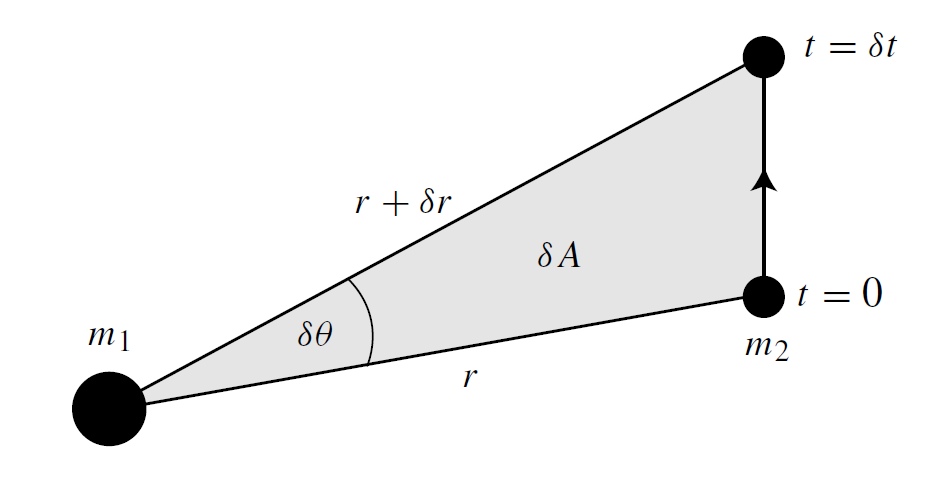
\includegraphics[width=0.3\textwidth]{Pic/Area_dynamics.png}
\caption{\cite{murray1999solar}}
\label{Area_dynamics}
\end{center}
\end{figure}

\begin{equation}
\delta A \approx \dfrac{1}{2} r(r+dr)\sin(\delta\theta) \approx  \dfrac{1}{2} r^{2}\delta\theta
\end{equation}

\begin{equation}
\dfrac{dA}{dt}=\dfrac{1}{2}r^{2}\dfrac{d\theta}{dt}=\dfrac{1}{2}h
\end{equation}

\begin{center}
$h$ is constant $\implies$ $2^{th}$ Kepler law
\end{center}


\end{frame}



\begin{frame}{Celestial mechanics \cite{murray1999solar}: $1^{th}$ Kepler law}
\begin{center}
Using the substitution $u=\dfrac{1}{r}$ $h=r^{2}\dot{\theta}$
\end{center}

\begin{equation}
\dot{r}=-\frac{1}{u}\dfrac{du}{d\theta}\dot{\theta}=-h\frac{du}{d\theta}
\end{equation}

\begin{equation}
\ddot{r}=-h\dfrac{d^{2}u}{d\theta^{2}}\dot{\theta}=-h^{2}u^{2}\frac{d^{2}u}{d\theta^{2}}
\end{equation}

\begin{equation}
\dfrac{d^{2}u}{d\theta^{2}}+u=\frac{\mu}{h^{2}}
\end{equation}

\begin{equation}
u=\frac{\mu}{h^{2}}\left[1+e\cos(\theta-\phi)\right]
\end{equation}

\end{frame}


\begin{frame}{Celestial mechanics \cite{murray1999solar}: $1^{th}$ Kepler law}
\begin{columns}
\column{0.5\textwidth}
\begin{equation}
r=\dfrac{p}{1+e\cos(\theta-\phi)}
\end{equation}


\begin{center}
$e$ is \textcolor{red}{eccentricity}
\end{center}

\begin{itemize}
\item circle:  $e=0$ \quad $p=a$
\item ellipse: $0<e<1$ \quad $p=b$
\item parabola: $e=1$ \quad $p=2q$
\item hyperbola: $e>1$ \quad $p=a(e^{2}-1)$
\end{itemize}
\begin{center}
$b$ is the  \textcolor{red}{semi-major axis} of the conic
\end{center}
\column{0.4\textwidth}
\begin{figure}[h]
\begin{center}
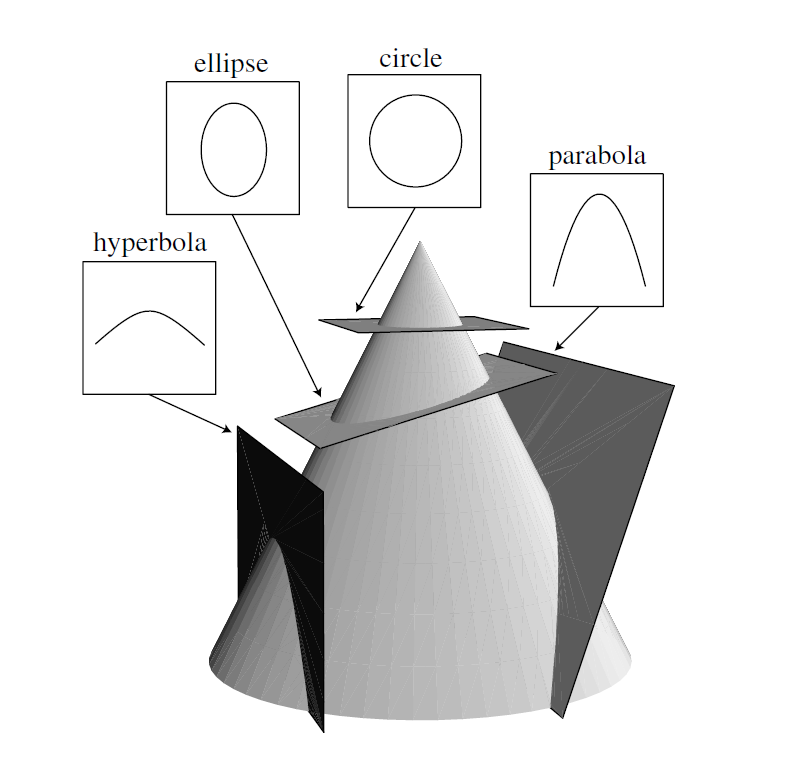
\includegraphics[width=\textwidth]{Pic/Conics.png}
\caption{\cite{murray1999solar}}
\label{Area_dynamics}
\end{center}
\end{figure}

\end{columns}
\end{frame}

\begin{frame}{Celestial mechanics \cite{murray1999solar}: $3^{th}$ Kepler law}
\begin{equation}
b^{2}=a^{2}(1-e^{2})
\end{equation}


\begin{equation}
r=\frac{a(1-e^{2})}{1+e\cdot cos(\theta-\phi)}
\label{eq-mot}
\end{equation}

\begin{center}
Area swept in one \textcolor{red}{orbital period} T $ \implies A=\pi ab$
We know that: $hT/2 \quad h^{2}=\mu a(1-e^{2})$ 
\end{center}

Therefore 

\begin{equation}
T^{2}=\dfrac{4\pi^{2}}{\mu}a^{3}
\end{equation}

\end{frame}

\begin{frame}{$3^{th}$ Kepler law}


\begin{equation}
\frac{m_{c}+m}{m_{c}+m'}=\left(\frac{a}{a'}\right)\left(\frac{T'}{T}\right)^{2}
\end{equation}

But since $m$,$m'<<m_{c}$

\begin{equation}
(a\a')^{3}\approx (T\T')^{2}
\end{equation}

And therefore 

\begin{equation}
T'\approx a'^{3/2}
\end{equation}


\end{frame}

\begin{frame}{Orbital parameters}
\begin{center}
\textcolor{red}{Mean motion}
\end{center}
\begin{equation}
n=\frac{2\pi}{T}
\end{equation}

\begin{equation}
v_{perihelion}=na\sqrt{\dfrac{1+e}{1-e}}
\end{equation}

\begin{equation}
v_{aphelion}=na\sqrt{\dfrac{1-e}{1+e}}
\end{equation}





\end{frame}



\begin{frame}{Orbital parameters}
\begin{center}
\textcolor{red}{Mean anomaly}
\end{center}
\begin{equation}
M=n(t-\tau)
\end{equation}

\begin{center}
\begin{itemize}
\item $M=f=0$\quad$t=\tau$\quad Perihelion
\item $M=f=\pi$\quad$t=\tau+T/2$ \quad Aphelion
\end{itemize}
\end{center}

\begin{equation}
M=E-e\sin E
\end{equation}

\begin{center}
\textcolor{red}{Jupiter Tisserard invariant }
\end{center}



\begin{equation}
T_{P}=\frac{a_{p}}{a}+2\cos I\sqrt{\dfrac{a}{a_{p}}(1-e^{2})}
\end{equation}

\end{frame}

\begin{frame}[t,allowframebreaks]
\frametitle{References}
\printbibliography
\end{frame}

\end{document}